
\documentclass[11pt,a4paper]{article}

\usepackage[utf8]{inputenc} 
\usepackage[T1]{fontenc} 
\usepackage{lmodern}
\usepackage{tcolorbox}


\usepackage[german]{babel}


\setlength{\parindent}{0pt}
\setlength{\parskip}{1ex plus 0.5ex minus 0.5ex}

\usepackage{amsmath} 


\usepackage{graphicx} 

\usepackage[section]{placeins}
\usepackage{booktabs}


\usepackage{hyperref}
\hypersetup{
	colorlinks,
	citecolor=red,
	filecolor=black,
	linkcolor=black,
	urlcolor=black}
\graphicspath{}

\begin{document}
	
	{
		\centering 
		\large 
		Physiklabor für Anfänger*innen \\
		Ferienpraktikum im Sommersemester 2018 \\[4mm]
		\textbf{\LARGE 
			Versuch 75: Lichtmikroskop
		} \\[3mm]
		(durchgeführt am 02.10.2018 bei Daniel Bartle) \\
		Ye Joon Kim, Marouan Zouari\\
		\today \\[10mm]
	}
	\tableofcontents
\newpage
\section{Einleitung}
Mit einer Lupe oder einem Mikroskop können kleine Objekte oder feine Einzelheiten stark vergrößert angesehen werden. Wie groß ein Objekt aussieht, hängt von dem Sehwinkel, $\epsilon =\arctan(B/b)$ ab (Siehe Abbildung 1). Eine Lupe lenkt das Licht so ab, sodass der Sehwinkel vergrößert wird. Deswegen mit einer Lupe sieht es so aus, als ob das Objekt größer geworden ist. Die Vergrößerung ist definiert durch:
\begin{equation}
V = \frac{\varepsilon}{\varepsilon_0}
\end{equation}

Wobei $\varepsilon_0$ und $\varepsilon$ jeweils der Sehwinkel ohne und mit der Lupe sind. Für sehr kleine Winkel gilt $\varepsilon \approx \tan(\varepsilon)$, und dadurch lässt sich $V$ auch schreiben als:
\begin{equation}
V \approx \frac{\tan\varepsilon}{\tan\varepsilon_0} = \frac{G/f}{G/s_0} = \frac{s_0}{f}
\end{equation}

Ein Mikroskop funktioniert ähnlich, aber es kann viel stärkere Vergrößerungen schaffen. Die zwei wichtigsten Teile eines Mikroskops sind das Objektiv und das Okular. 

Das Licht von dem Objekt geht zuerst durch das Objektiv. Das Objektiv bricht das Licht so, sodass es am Brennpunkt des Okulars ein vergrößertes reelles Zwischenbild entsteht. Das Okular schickt, wie eine Lupe, das Licht in das Auge, wobei das Bild nochmals vergrößert wird (Siehe Abbildung 2). Mit nur diesen zwei Linsen können riesige Vergrößerungen geschafft werden. Die Gesamtvergrößerung eines Mikroskops kann mit der folgenden Formel geschrieben werden:
\begin{equation}
V_\textrm{Mikroskop} \approx \frac{\tan\epsilon}{\tan\epsilon_0}= \frac{B/f_2}{G/s_0} = \frac{B}{G}\cdot\frac{s_0}{f} = \beta_\textrm{obj}\cdot V_\textrm{ok}
\end{equation}
Wobei $B$ und $G$ die jeweils Bild- und Gegenstandgröße bezüglich des Objektives, $\beta_\textrm{obj}$ der Abbildungsmaßstab des Objektives und $V_\textrm{ok}$ die Vergrößerung des Okulars sind. 


\begin{figure}
	\centering
	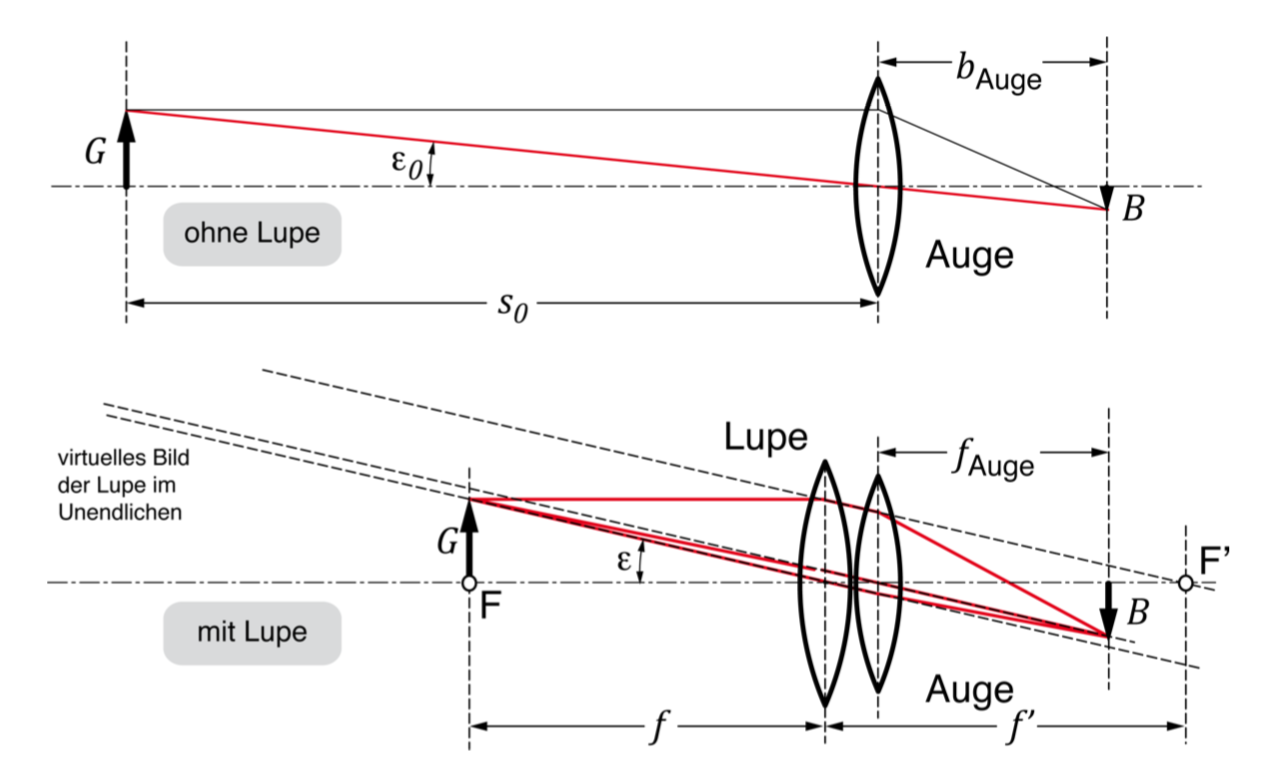
\includegraphics[width=\linewidth]{Abb1}
	\caption{Funktionsweise einer Lupe (,,Versuchsanleitungen'')}
\end{figure}

\begin{figure}
	\centering
	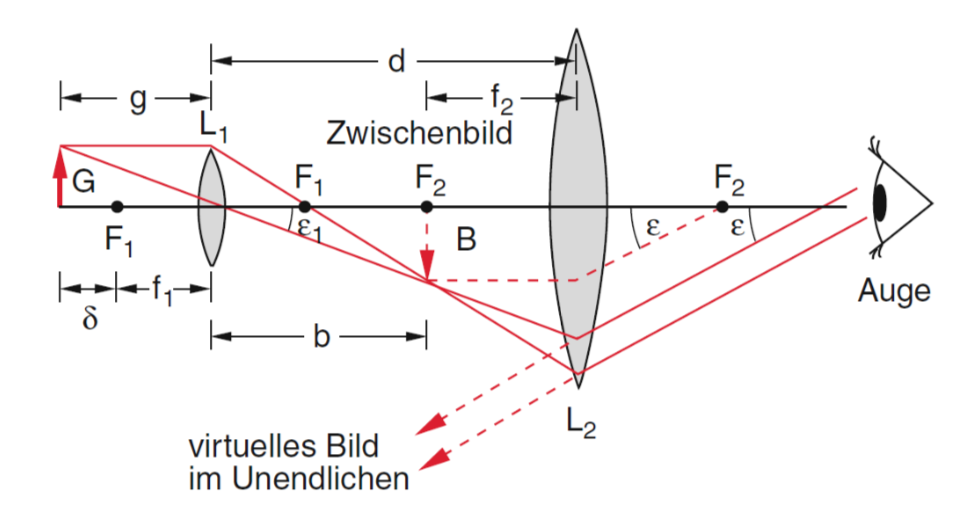
\includegraphics[width=\linewidth]{Abb2}
	\caption{Funktionsweise eines Lichtmikroskops(,,Versuchsanleitungen'')}
\end{figure}

Bei echten Mikroskope sind aber nicht nur die Vergrößerung aber auch die Beleuchtung wichtig. In diesem Versuch wird die Köhlersche Beleuchtung untersucht. Zu dem werden vier zusätzliche Bauteilen benötigt. 

Die Kollektorlinse bildet die Lichtquelle vergrößert auf die dahinten stehende Leuchtfeldblende ab. Der Hebel von der Leuchtfeldblende kann verstellt werden, um die Größe der Apertur zu ändern, und dadurch kontrolliert die Blende wie groß die Abbildung auf dem Schirm ist. Daneben steht eine Aperturblende, die sich an dem Brennpunkt der dahinten stehenden Kondensorlinse befindet. Ähnlich wie die Leuchtfeldblende kann die Größe des Lochs an der Blende justiert werden, aber da die Blende sich am Brennpunkt der Kondensorlinse befindet, wird nicht die Größe sondern nur die Helligkeit der Abbildung beeinflusst. Die Kondensorlinse bildet dann das Licht auf das Objektebene (Siehe Abbildung 3).

Bei Mikroskope ist auch seine Auflösung wichtig. Mit Auflösung bezeichnet man den kleinsten Abstand zwei Punkte dazwischen haben müssen, sodass beide Punkte voneinander unterscheidet werden können, und dies hängt von der Größe der Öffnung des Mikroskops ab. Dieser Abstand kann mit der folgenden Formel berechnet werden (in Luft):
\begin{equation}
\delta = \frac{1,22\lambda}{2 \sin \alpha}
\end{equation}
Wobei $\lambda$ und $\alpha$ jeweils die Wellenlänge des Lichts und die halbe Öffnungswinkel sind. 

Das Ziel des Versuchs ist deshalb es, der Abbildungsmaßstab des Objektivs, die Vergrößerung des Okulars und des gesamten Mikroskops und die Auflösungsbegrenzung mit einem Objektmikrometer zu messen. 

\begin{figure}
	\centering
	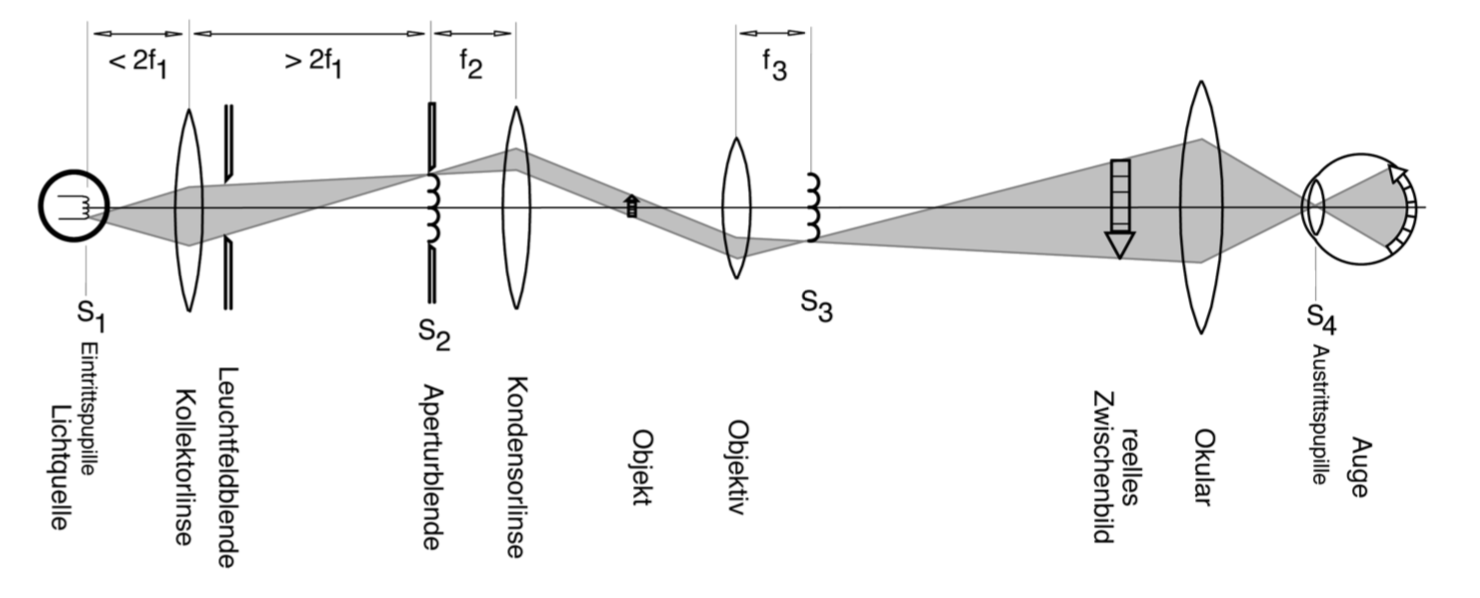
\includegraphics[width=\linewidth]{Abb3}
	\caption{Köhlersche Beleuchtung und Versuchsaufbau (,,Versuchsanleitungen'').}
\end{figure}

\section{Aufbau}
Zum Versuch wurden die in dem obigen Abschnitt erwähnten optische Apparate, eine optische Bank, ein transparenter und opaker Schirm mit ein Stück Millimeterpapier, eine beleuchtete Referenzskala und zwei Objekte (Drahtgitter und Objektmikrometer) benutzt (Siehe Abbildung 3). 

\section{Durchführung}
Es wurden zuerst auf der optischen Bank der Schirm und Objektivelinse fixiert. Die Linse und Schirm wurden so verschoben, sodass es eine relativ scharfe vergrößerte Abbildung auf dem Schirm erzeugt wurde. Die Lichtquelle wurde justiert, sodass die Abbildung zentriert war.  

Für den ersten Versuchsteil wurde ein Drahtgitter vor dem Objektiv bei Position 250mm eingesetzt. Das Objektiv wurde dann verschoben, damit eine scharfe Abbildung des Gitters entstanden war. Dann wurde eine Kollektorlinse direkt vor der Lichtquelle fixiert. Ihre Position wurde variiert und der Einfluss auf die Beleuchtung wurde beobachtet. Die Aperturblende wurde dann zwischen dem Objekt und der Kollektorlinse eingesetzt. Es wurde dann untersucht am welcher Stelle der ausgeleuchtete Bereich nicht geändert wurde, wenn die Aperturblende gedreht wurde. Eine Leuchtfeldblende wurde dann zwischen der Aperturblende und Kollektorlinse fixiert und es wurde untersucht ob die Position der Kollektorlinse einen Einfluss auf die Beleuchtung hat. 

Für den zweiten Teil wurden die Bauteile ein Bisschen justiert, um das Objekt optimal abbilden zu können. Die Kollektorlinse wurde am Position 11,5 cm, die Leuchtfeldblende am Position 12,7 cm, die Aperturblende am Position 19,2 cm, die Kondensatorlinse am Position 25,0 cm, das Objekt am Position 30,7 cm, das Objektiv am Position 35,8 cm und der Schirm am Position 119,0 cm fixiert. Für das Objekt wurde der Objektmikrometer ausgewählt. Die Größe einer abgebildeten Skala wurde dann mit der Millimeterpapier auf dem Schirm gemessen. Danach wurden die Abstände zwischen dem Objekt und Objektiv und dem Bild und Objektiv gemessen. 

In dem dritten Versuchsteil wurde das Okular 50 mm hinter dem Schirm fixiert und der Würfel direkt dahinter. Der Schirm wurde umgedreht, sodass das Millimeterpapier auf der rechten Seite des Schirms sich befand. Die Referenzskala wurde dann 120 mm hinter dem Würfel eingesetzt. Der Auge wurde 2 cm oberhalb des Würfels gebracht, und der Referenzskala wurde verschoben, sodass beide Skalen gleichzeitig sichtbar waren. Die Größe einer Skala des abgebildeten Millimeterpapiers wurde dann mit dem reflektierten Bild der Referenzskala gemessen. 

Für den vierten Versuchsteil wurde der opake Schirm durch die transparente Mattscheibe ersetzt. Die Größe einer auf die Mattscheibe abgebildeten Skala wurde dann wie in dem dritten Versuchsteil mit der Referenzskala gemessen. 

Für den fünften Versuchsteil wurde ein Spalt nah hinter dem Objektiv fixiert, und die Mattscheibe durch den weißen Schirm ersetzt. Der Schirm wurde so positioniert, sodass eine scharfe Abbildung des Objektmikrometers auf dem Schirm entstanden war. Die Spaltbreite wurde dann verringert, bis die abgebildeten Skalen nicht mehr voneinander unterscheidet werden konnten. Das Objekt wurde dann durch den Spalt ersetzt, und die Größe des abgebildeten Spalt wurde dann mit einem Lineal gemessen. 

In dem sechsten Versuchsteil wurde das Drahtgitter als Objekt ausgewählt. Es wurde dann beobachtet, ob es Abbildungsfehler gab. 


\section{Auswertung und Fehleranalyse}
\subsection{Bestimmung der Abbildungsmaßstab des Objektivs}
Der Abbildungsmaßstab ist definiert als:
$$ \beta = \frac{B}{G} = \frac{b}{g} $$
Wobei $B$ und $G$ jeweils die Bild- und Gegenstandgröße und $b$ und $g$ jeweils die Bild- und Gegenstandsweite sind. Der mit den Bild- und Gegenstandgröße bestimmte Abbildungsmaßstab und seine Unsicherheit sind:
$$ \beta = 20,0 \pm 1,4 $$
und der mit den Bild- und Gegenstandsweite bestimmte Abbildungsmaßstab:
$$ \beta = 15,5 \pm 0,3 $$

Für die Unsicherheiten wurde die vereinfachte gaußsche Fehlerfortpflanzung für Produkte benutzt. Die Unsicherheit des Abbildungsmaßstabs ist deshalb:
$$ \frac{\Delta \beta}{\beta} = \sqrt{\left(\frac{\Delta B}{B}\right)^2+\left(\frac{\Delta G}{G}\right)^2}$$
und ebenfalls mit den Bild- und Gegenstandsweite. 

\subsection{Bestimmung der Vergrößerung des Okulars}
Die Vergrößerung des Okulars wurde dadurch berechnet, indem man die Größe der gemessenen Referenzskalen durch die tatsächliche Größe der Skalen auf dem Millimeterpapier teilt. Die Vergrößerung und ihre Unsicherheit ist deshalb:
$$ V = 2 \pm 0,2 $$ 

Die Unsicherheit wurde wiederum mit der vereinfachten gaußschen Fehlerfortpflanzung berechnet, deswegen:
$$\frac{\Delta V}{V} = \sqrt{\left(\frac{\Delta B_1}{B_1}\right)^2+\left(\frac{\Delta B_2}{B_2}\right)^2}$$
wobei $B_1$ und $B_2$ jeweils die Größe der gemessenen Referenzskalen und die tatsächliche Größe der Skalen auf dem Millimeterpapier sind. 

\subsection{Bestimmung der Vergrößerung des gesamten Mikroskops}
Die Vergrößerung des gesamten Mikroskops und ihre Unsicherheit wurden ebenso berechnet:
$$V_\textrm{tot} = 70 \pm 20$$

Zum Vergleich kann ein halb-theoretischer Wert dafür mit den vorher gemessenen Abbildungsmaßstab und Vergrößerung des Okulars bestimmt werden. 

$$V_\textrm{Tot Theo} = 40 \pm 5$$

Die Unsicherheit davon wurde mit der gaußsche Fehlerfortpflanzung für Produkte berechnet. 

$$\frac{\Delta V_\textrm{Tot Theo}}{V_\textrm{Tot Theo}} = \sqrt{\left(\frac{\Delta V}{V}\right)^2+\left(\frac{\Delta \beta}{\beta}\right)^2}$$
  
\subsection{Bestimmung der Größe des Spalts}
Die Größe eines Gegenstands lässt sich mit seiner abgebildeten Größe und dem Abbildungsmaßstab bestimmen. Nämlich:
$$ G = \frac{B}{\beta}$$
Die Größe des Spalts ist deshalb:
$$ s = 0,050 \pm 0,004 \textrm{cm}$$
Die Unsicherheit wurde fast genau wie in den obigen Teilen mit der vereinfachten gaußschen Fehlerfortpflanzung berechnet. Für $\beta$ wurde der erste Wert ausgewählt, da er wurde direkt gemessen. 

Um der theoretische kleinste auflösbare Abstand zu bestimmen, wurde Gleichung (4) benutzt. Für die Wellenlänge wurde die durchschnittliche Wellenlänge von dem Lichtspektrum ausgewählt (545 nm), da weißes Licht enthält Licht von allen Farben (,,Visible Spectrum''). Mit $\alpha \approx \frac{s}{f}$ ist dieser Abstand:
$$\delta \approx 0,0026 \textrm{mm}$$


\section{Diskussion der Ergebnisse}
Die zwei gemessenen Werte für den Abbildungsmaßstab des Objektivs sind:
$$ \beta_{B/G} = 20,0 \pm 1,4$$
$$ \beta_{b/g} = 15,5 \pm 0,3$$
Um zu sehen ob diese zwei Werte miteinander verträglich sind, wurde ihr $t$-Wert berechnet mit:
\begin{equation}
t = \frac{|\beta_{B/G}-\beta_{b/g}| }{\sqrt{u_{\beta_{b/g}}^2+u_{\beta_{B/G}}^2}}
\end{equation}
was $t\approx3,14$ beträgt. Da dieser Wert größer als 2 ist, sind diese zwei Werte miteinander nicht verträglich. Der erste Wert ist trotz der größeren Unsicherheit mehr signifikant und Bedeutungsvoll, da es wurde direkt gemessen. 

In dem zweiten Versuchsteil wurde die Vergrößerung des Okulars bestimmt. 

$$V_\textrm{Ok} = 2 \pm 0,2$$

Da es keinen angegebenen oder theoretischen Wert für die Vergrößerung gibt, kann es nicht beurteilt werden, ob dieser Wert akkurat ist. Dieser Wert besitzt aber eine große relative Unsicherheit (10\%), deswegen ist dieser Wert nicht sehr aussagekräftig. 

In dem dritten Teil wurde die Gesamt-Vergrößerung des Mikroskops bestimmt:
$$V_\textrm{tot} = 70 \pm 20$$

Die theoretische und gemessene Gesamt-Vergrößerung des Mikroskops wurde ebenso verglichen. Ihr $t$-Wert lautet:
$$t = 1,45 $$
Da dieser Wert kleiner als 2 ist, sind diese zwei Werte miteinander verträglich. Dieses Ergebnis ist aber nicht sehr signifikant, da die relative Unsicherheit von $V_\textrm{tot}$ fast 30\% beträgt.

In dem letzten Versuchsteil wurde die Größe des Spalts, wobei die einzelnen Skalen des abgebildeten Objektmikrometer voneinander nicht unterscheidet werden konnten, bestimmt:
$$s = 0,050 \pm 0,004 \textrm{cm}$$

Da die relative Unsicherheit ungefähr 10\%, beträgt, ist dieser Wert auch nicht sehr aussagekräftig. 

Die theoretische Auflösung lautet:
$$\delta \approx 0,0026 \textrm{mm}$$
was ungefähr dreimal des Abstands zwischen den Skalen waren. 
\subsection{Systematische und Statistische Fehler}
Ein systematischer Fehler ist es, dass der Wert für $\beta$, der auch bei anderen Berechnungen benutzt wurde, selbst wegen der Unsicherheit eine Abweichung von dem wirklichen Wert hat. Deswegen können alle Werte, die mithilfe dieses Werts berechnet wurden, in einer Richtung von den wirklichen Werte verschoben sein. 

Ein statistischer Fehler war es, dass es schwierig war, die genauen Lagen der Linse und anderen Bauteile, wobei eine scharfe Abbildung möglich war, zu bestimmen, da wie scharf eine Abbildung aussieht musste mit bloßem Auge qualitativ beurteilt werden. Dieses Problem lässt sich dadurch lösen, indem man ein Gerät benutzt, das automatisch bestimmen kann, wann ein Bild am schärfsten ist (Wie die Autofokus-Funktion bei einer Kamera). 
\subsection{Vergleich mit einem kommerziellen Mikroskop}
Im Vergleich mit einem kommerziellen Mikroskop hat das selbstgebaute Mikroskop eine kleinere Vergrößerung und schlechtere Beleuchtung. Deswegen ist es mit dem kommerziellen Mikroskop viel leichter, feine Einzelheiten oder kleinere Objekte anzusehen. Das kommerzielle Mikroskop ist auch viel kompakter, und daher ist es praktisch und nützlich. 


\section{Literatur}
,,Versuchsanleitung zum Physiklabor für Anfänger*innen.'' Albert-Ludwigs-Universität Freiburg. 

,,Visible Spectrum.'' Wikipedia. 
\section{Anhang}
(Siehe Scans)

\end{document}